\chapter{Topic Extraction Engine}

The semantic analysis tool focused on 2 main text mining components in order to extract information from the news articles. This section focuses on the first of these components: the topic extraction engine, covering different data processing techniques, word and document approaches, semantic clustering and topic modelling using LDA. 

\section{Data Processing} \label{procesing_topic}

The prepared data (from Section \ref{dataloader}) grouped by (Year, Category) comprised of a list of articles that were published in that year and assigned that category. Processing all the text for every single article would add an intensive computational burden without a huge amount of added benefit, with a potential risk of cluttering the model. For the sake of brevity, the aim was to use the article data most representative of the article. To facilitate this, a decision was made to use the titles and introduction of the articles as they contain the core information in the articles. The introduction of the article (`intro') was extracted as the first \hl{6} sentences of the article using SpaCy's \texttt{SentenceSplitter}. Throughout the \hl{course of this report}, `intro' and `article' will be used inter-changeably to represent a single news article in the corpus. 

Once the article introductions are extracted, they then undergo pre-processing before they can be vectorised for clustering. This section highlights the different pre-processing steps and key decisions made to convert the article intros into a list of tokens for the vectorisation step.

\subsection{Coreference Resolution} \label{coref}
The first step involves coreference resolution of the articles (`intros'). This involves using the pre-trained AllenNLP SpanBERT coreference resolution model for finding the set of mentions in the text that refer to the same `entity' (i.e. coreference clusters). This step was performed on the complete article intro in order for the mentions to be resolved throughout the entirety of the intro and not just on a sentence level. For example, for the text `Sean Doyle is the CEO of British Airways. Prior to this, he was the CEO of Air Lingus', if the coreference resolution was done on the sentence level, the model would miss out on resolving `he' in the second sentence to `Sean Doyle'.

\subsection{Cleaning Data} \label{data_cleaning}
Post coreference resolution of the article intros, the data needed to be `cleaned' in order to ensure that the news articles retrieved were informative and useful. This involved the following steps: 
\begin{enumerate}
    \item Removing any unnecessary characters e.g., trailing ellipsis, parenthesis etc.
    \item Removing stopwords. The spaCy model's default stopwords list was used. This significantly reduced the amount of text per article intro by removing words such as this, `that', `there', `where', `are' etc. This alone, however, was not sufficient. Given the nature of online news articles, there were some prominent phrases that showed up in several articles, e.g., \qd{Read here}, \qd{For more information}, \qd{Sourced by} etc. These were also removed as they do not provide any relevant information specific to the article, thereby reducing redundancy.

\end{enumerate}

\subsection{Removing Named Entities}
As mentioned previously, the aim of these pre-processing steps was to obtain a \texttt{filtered\_tokens} list for each article intro which would be vectorised to represent an article as a vector for clustering. 
One of the key decisions made was to remove all corresponding named entities extracted using the fine-grained Named Entity Recognition model from each article intro. This was done in order to remove any dependency of the topics on the named entities in the articles for clustering and topic modelling. Eliminating this dependency results in better silhouette scores and coherence scores for semantic clustering and topic extraction as detailed in Section \ref{s:preprocess_clustering} and \ref{s:preprocess_topic} respectively. Additionally, this step was done before tokenisation as named entities can often be a collection of words such as ``British Airways", ``Paul Sweeney", ``New Haven" etc. and removing these post-tokenisation would not be ideal as they would lose their semantic meaning as tokens. For instance, post tokenisation, the model would try to remove ``New", `Haven" from the article intro. Therefore, regex patterns were used to remove all the occurrences of the extracted entities in an article. This included removing all entity types which included but were not limited to, `PER', `LOC', `DATE', `ORG'. This also had a performance gain over the post-tokenisation approach as it avoided the lookup for each token against the unwanted entity tokens list.

\subsection{Filtering Tokenised Data} \label{filtered_tokens}
Once the data was cleaned and void of the pre-determined entity types, the article intros were tokenised and normalised. This was done using the SpaCy library's \texttt{Tokeniser} and \texttt{Lemmatiser} pre-trained on the English language model: \hl{en\_core\_web\_lg} (refer to Section \ref{libraries}). Normalisation was done through lemmatisation (to obtain the base forms of the tokens). This was chosen instead of stemming as it guaranteed more semantically meaningful tokens which for reasons detailed in Section \ref{normalisation}. The process of obtaining a list of tokens for each article intro was as follows:
\begin{enumerate}
    \item Each sentence in the intro was turned into a list of tokens.
    \item These tokens were filtered by their Part-Of-Speech (POS) tags against the allowed POS tags, which was restricted to nouns (`NOUN').
    \item Tokens that were numeric and less than 2 characters were also removed. 
    \item The remaining tokens were lemmatised and added to the \texttt{filtered\_tokens} list for the given article.
\end{enumerate}

It is important to note that the allowed POS tags were originally set to include nouns (NOUN), adjectives (ADJ), verbs (VERB) and adverbs (ADV) . This resulted in a lot of unnecessary tokens such as ‘because’, ‘did’, ‘very’ etc. Different combinations of the allowed POS tags were experimented with, ultimately allowing only nouns to comprise the \texttt{filtered\_tokens} for each article (`intro'). This decision was primarily based on the resulting clustering scores when the allowed POS tags were limited to `NOUN' and when they included `NOUN', `ADJ', `VERB' and `ADV' as discussed in the evaluation in Section \ref{s:pos_clustering}.

\section{Generating Document Vectors}

Once the corresponding \texttt{filtered\_tokens} list for each article intro is obtained, the individual tokens are vectorised, so they can be used to generate the document vectors.

\subsection{Word embedding approaches} \label{word_embed_approaches}
To vectorise the tokens, different pre-trained word embedding models were used. These approaches (in chronological order) with their strengths and shortcomings are outlined below.

\renewcommand\arraystretch{2}
\captionsetup{singlelinecheck=false, labelfont=sc, labelsep=quad}
\begin{longtable}{@{\,}r <{\hskip 2pt} !{\foo} >{\arraybackslash}p{13cm}}
\centering

TF-IDF & Term frequency-inverse document frequency is a statistical metric that examines the comparative relevance of a word/token with respect to an article intro in the collection of articles. Representing the tokens as their TF-IDF measure first involves calculating the term frequency (TF) using the bag of words (BoW) approach from Gensim \texttt{Doc2BoW}. To account for overlapping terms across all article intros, the term frequency was multiplied by the inverse document frequency to weigh down the terms whose high frequency is not unique to a document (Refer to  \hl{Add in BCKG}). A dense document-term using the TF-IDF values for each term is used to represent the article intro as a vector for clustering. \\

Word2Vec & The next approach saw the use of Google's \texttt{Word2Vec} model (from Gensim) to obtain pre-trained word embeddings for each token in an article's corresponding \texttt{filtered\_tokens} list. The issue with the previous approach was that it represented the statistical information about a document, in particular, the measure of the frequency of words in a document, rather than any semantic information about a document. \texttt{Word2Vec} embeddings, on the other hand, return a vector for each word that accounts for semantic similarity (based on cosine distance) between the words represented by the vectors \cite{word2vec}.   \\

GloVe & The final approach was to use Stanford’s \texttt{GloVe} (global vector) embeddings from Gensim. \texttt{GloVe} as been pre-trained on Wikipedia and Gigaword 5, comprising of a vocabulary of 400,000 words which are represented by 300 dimensional vectors \cite{glove}. The advantage of this approach over previous approaches is that it makes use of global statistics such as word co-occurrences to obtain word vectors. Using these embeddings also saw an improvement in the silhouette scores when deriving the semantic clustering of articles as detailed in Section \ref{s:word_embeddings}. \\
\end{longtable}

\subsection{Document embeddings}

In Section \ref{filtered_tokens}, \texttt{filtered\_tokens} are defined as the all \textit{relevant} tokens for each article intro. As mentioned above, the filtered tokens were vectorised using the \texttt{GloVe} embeddings \cite{glove} resulting in a list of vectors corresponding to the \texttt{filtered\_tokens}. In order to get the document vectors from these word vectors, two approaches were tested: 

\renewcommand\arraystretch{2}
\captionsetup{singlelinecheck=false, labelfont=sc, labelsep=quad}
\begin{longtable}{@{\,}r <{\hskip 2pt} !{\foo} >{\arraybackslash}p{13cm}}
\centering

Approach 1 & The corresponding tokens in \texttt{filtered\_tokens} list for the article intro are vectorised (using \texttt{GloVe} embeddings) and averaged to find the corresponding article vector. This was a simple approach that gave equal importance to each token associated with the article intro. \\

Approach 2 & Rather than simply averaging the token vectors for each article intro, the document vector was calculated using a weighted sum of corresponding word vectors (from \texttt{filtered\_tokens}). This was done by using a TF-TDF model to get the term-frequency inverse document frequency weight for each token in the corresponding article. This meant that words that appeared in high frequency unique to the associated article contributed more to the document vector than those with a lower frequency or those that appeared frequently in other article intros. \\
\end{longtable}
%%%%%%%%%%%%%%%%%%%%%%%%%%%%%%%%%%%%%%%%%%%%%%%%%%%%%%%%%%%%

\todonum[inline]{Add the document graph}

\section{Semantic Clustering}

Once the article intro vectors are calculated, they are processed so they can be used for semantic clustering. 

\subsection{Dimensionality Reduction}

\subsubsection{Normalising Data}
The first step is to normalise the article vectors in order to eliminate redundancy in data and standardise the features (components of the vector) in case of high variance, which contributes to better clustering. Additionally, when it comes to performing principal component analysis for the article vector, we want the features (in vectors) to be independent of their standard deviation or variance. This is necessary to get a good covariance matrix among the features.  

\subsubsection{Principal Component Analysis}

As established previously (refer to Section \ref{word_embed_approaches}), \texttt{GloVe} document embeddings result in a 300-dimensional vector. Clustering the document vectors becomes inefficient and meaningless at these high dimensions as the concept of distance becomes less precise as the number of dimensions increases \cite{pca_clustering} as the volume of space increases exponentially making the available data spare - curse of dimensionality. For any given point in this high n-dimensional space, the difference in 'distance' (euclidean) to the closest point $d_min$ and the farthest point $d_max$ with respect to the $d_min$ becomes negligible \cite{nearest_neighbour}. 

\[ \lim_{n\to\infty} \frac{d_{max} - d_{min}}{d_{min}} \to0\]

The concept of clustering these articles relies on grouping similar articles together based on their attributes. The similarity is determined based on the vectorised \texttt{filtered\_tokens}. However, given the high dimensional nature, some of these attributes will not be relevant in determining these clusters. The goal is to find the attributes (vector components) with the most variance across the documents vectors to represent the features. This is accomplished by performing principal component analysis (PCA) on the normalised high-dimensional input vector space to map to a low dimensional space, whilst minimising information loss \cite{pca_clustering}.

\begin{figure}[H]
  \centering
  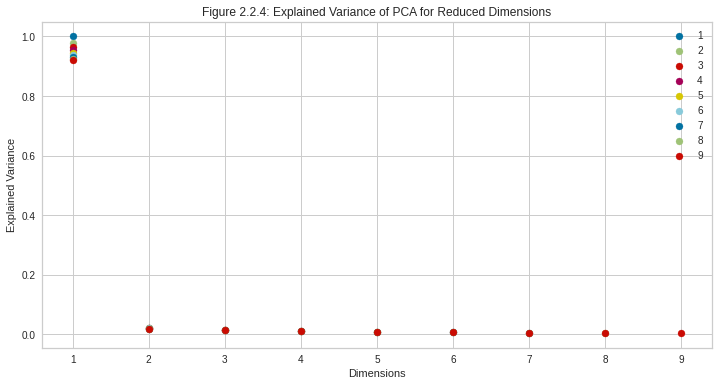
\includegraphics[scale=0.3]{images/explained variances.png}
  \caption{Explained Variances for PCA for dimensions=1..9 }
  \label{fig:pca}
\end{figure}

\hl{TODO: sil scores with different pca? or explained variances?} 

\subsection{KMeans Clustering}
Once the normalised data is mapped to the lower subspace, the documents (article intros) are clustered based on similarity. The aim is to cluster the article intro vectors based on their cosine similarity (Eq. \ref{eq:cosine_sim}) using cosine distance as the distance function (Eq. \ref{eq:cosine_distance}). The clustering technique used was KMeans clustering. This was done using the \texttt{sklearn} library's \texttt{kmeans} function with `euclidean distance' (Eq. \ref{eq:euc_distance}). This was feasible given the linear relationship between Euclidean distance and  cosine distance \cite{kmeans} for normalised vectors as in shown in Eq. \ref{eq:relationship_ce}.


\begin{align}
  \mathit{For \ normalised \ vectors,} \ x, y:  \sum x_i^2 &= 1,  \sum y_i^2 = 1 \label{eq:normalised} &\\ 
  \mathit{Cosine \ Similarity,} \ cos(x, y) &= \frac{\sum x_i y_i}{\sqrt{\sum x_i^2 y_i^2}}  \nonumber &\\ 
   &= \sum x_i y_i \label{eq:cosine_sim} &\\
   \mathit{Cosine \ Distance} &= 1 - cos(x, y) \label{eq:cosine_distance} &\\
   \mathit{Euclidean \ Distance,} \ || x - y ||_2^2  &= \sum (x_i -  y_i)^2  \label{eq:euc_distance} &\\
                 &= \sum (x_i^2 + y_i^2 - 2 x_i y_i)  \nonumber &\\
                 &= \sum x_i^2 + \sum y_i^2 - 2\sum x_i y_i   \nonumber &\\
                 &= 1 + 1 - 2 cos(x, y)  \nonumber &\\
                 &= 2 (1 - cos(x, y))  &\\
                 &= 2 (\mathit{Cosine \ Distance}) \label{eq:relationship_ce}
\end{align}


% \todonum[inline, color=darkgray]{Add kmeans formula - MDS?}

Furthermore, to avoid falling into the trap of random centroids initialization, which is a major shortcoming of the KMeans method, the clustering was done with KMeans++. The reason for doing so was that KMeans++ offers a better initialisation approach for centroids, in which the first one is picked at random and the subsequent centroids are chosen with a probability proportional to the squared distance from the closest chosen centroid.


\subsection*{Finding the optimal number of clusters: k}
Determining the number of clusters (k) in KMeans is a crucial factor to consider. This was done by computing the KMeans clustering algorithm for different values of k varying from 2 (minimum number of clusters) to m (maximum number of clusters), and picking the optimal k based on a comparing statistic. The two comparison statistics considered were: Elbow method with Wihtin Cluster Sum of Square distance (WCSS) and silhouette score. 

\subsubsection{Method 1: Elbow method}
The elbow method uses the distance (Euclidean) between the cluster centroid and its members, i.e., intra-cluster variance (distortion score or WCSS) to determine how many clusters are needed to encapsulate the variance of the data. In particular, it minimises the loss function: WCSS (a.k.a. distortion score) which is the sum of the squared distance between each point and the centroid in a cluster \cite{elbowvssil}.

\begin{align}
  \mathit{WCSS} &=  \sum^{C_n}_{C_k} (\sum^{d_m}_{d_i \in C_i} || d_i - C_k ||_2^2) \label{eq:wcss}
\end{align}

As seen in Figure \ref{fig:elbow}, the elbow (bend) in the plot determines the optimal number of clusters, i.e., the k value = 5. After this value, distortion score gives diminishing returns.

\begin{figure}[H]
\centering
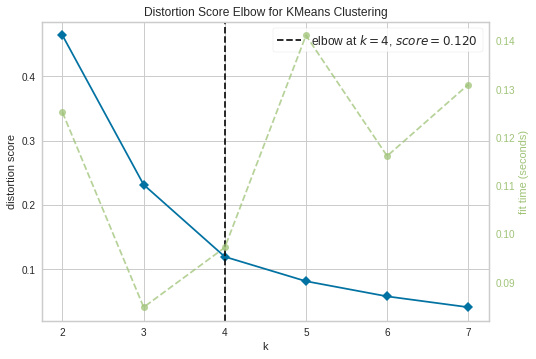
\includegraphics[scale=0.5]{images/elbow.png}
\caption{Elbow score: Elbow Method Plot for ('Business', 2020) for k=2 to 12}
\label{fig:elbow}
\end{figure}

\subsubsection{Method 2: Silhouette score}

The second approach involved using the silhouette score. Unlike, the elbow method silhouette score combines both separation and cohesion \cite{elbowvssil}. This means it means how close a point is within its cluster (cohesion) and other clusters (separation) \cite{silhouette}.

\begin{center}
    $\mathit{Silhouette \ Score }= \mathit{mean}_i (\frac{S_i - C_i}{\max(S_i, C_i)}) $
\end{center}
% \ mathrm
where 
cohesion, $C_i$ = average distance between i and all points within its cluster.
separation, $S_i$ = average distance between i and all points not in its cluster.

The silhouette score is the mean of Sil(i) for all points i in the data. It ranges from -1 to 1. A value closer to 1 indicates that clusters are well separated and distinguished. A value very close to 0 indicates there is significant overlapping between the clusters, and the clusters are not distinguished. A value near -1 indicates that clusters are assigned incorrectly.

Out of these two approaches, I decided to go with the silhouette score as it gives a better value of the goodness of a clustering. It factors both how compact a cluster is and how distinct it is. Additionally, it is better suited for large volumes of data and given that in the context of the problem, the aim is to cluster the news articles into distinct clusters with little overlap, as o each of these clusters, topic modelling will be performed to extract topics and ideally, there should very few common topics among the clusters.

\begin{figure}[H]
\begin{minipage}{0.5\linewidth}
\centering
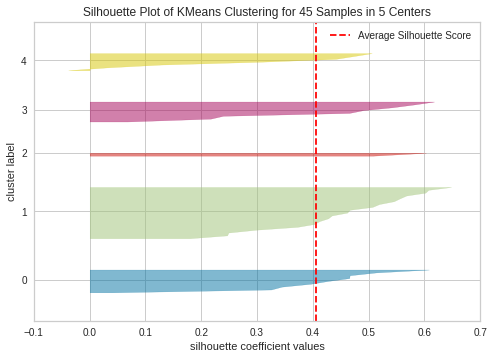
\includegraphics[width=\linewidth]{images/cluster 5.png}
\caption{Silhouette score = 0.4059555 for Kmeans clustering k=5, for (’Business’, 2020)}
\end{minipage}
\hfill
\begin{minipage}{0.48\linewidth}
\centering
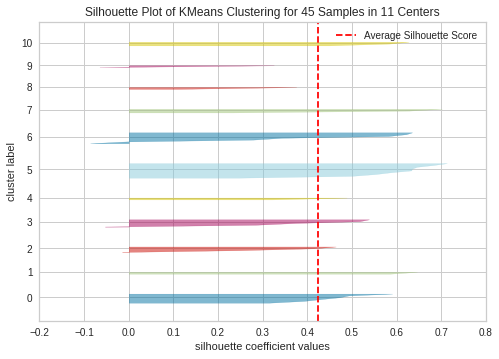
\includegraphics[width=\linewidth]{images/cluster 11.png}
\caption{Silhouette score = 0.4229686 for Kmeans clustering k=11, for (’Business’, 2020)}
\end{minipage}
\end{figure}

We can see in the plots generated by YellowBricks machine learning visualization library in Figure \hl(???) that the optimal cluster number, k = 5 (from Figure \hl{???}) chosen by the Elbow Method is not the same as the one chosen by the silhouette method k = 11.
\todonum[inline, color=darkgray]{Add explanation}
% Fig 3. K-means clusters Silhouette Plot for n_clusters = 4 (Below Avg Score)
% Whether there is wide fluctuations in the size of the cluster plots. If there are wider fluctuations like the following, the number of cluster is sub-optimal. In the diagram below, you could see wide fluctuations with one cluster below average score, other is very large and yet another ones in between. Thus, the choice of n_clusters = 5 will be sub-optimal.

% Fig 4. K-means clusters Silhouette Plot for n_clusters = 5 (Wide fluctuations)
% Whether the thickness of the clusters’ Silhouette plot is uniform. If there are clusters of non-uniform thickness, the number of clusters is sub-optimal. In the diagram below, you will see the two cluster Silhouette plots to have non-uniform thickness, one being very much thicker than another. Thus, the choice of n_clusters = 2 will be sub-optimal.

% Fig 5. K-means clusters Silhouette Plot for n_clusters = 2 (Nonuniform Thickness)
% Given above, the Silhouette plot for n_clusters = 3 looks to be most appropriate than others as it stands well against all the three measuring criteria (scores below average Silhouette score, Wide fluctuations in the size of the plot, and non-uniform thickness). Here is how the plot looks like:

\subsection{Find n most representative docs}
\label{sec:Find_n_docs}
Once the article intros are clustered, we want to obtain a cluster to article mapping. However, with volumes of data, it may not be as unnecessary to consider every single article in the cluster particularly those that are not close to their respective cluster centroids. More importantly, since the next step is topic modelling on these clusters of article intros, we do not want to consider those clusters that have very few members as they will not spawn any good topics. In order to facilitate this, the idea of using the n most representative articles comes to play. \\

A pre-determined value n is selected and for each cluster, the euclidean distance of each member (article intro) in the cluster is compared with its centroid. The articles are sorted in decreasing order of distance and the top n articles are selected.\\

The question to consider then is how to decide this value of n. 
This value of n is calculated based on the clustering. First, the range of the size of clusters is calculated with the minimum number of data points (i.e, article intros) in a cluster subtracted from the maximum number of data points in a cluster. Then, the average number of data points in clusters is calculated. The minimum of the these two values determines n. This is done so that sparse clusters are omitted from the input data for topic modelling. This gives a final mapping of cluster to article intros (pruned).\\

\todonum[inline, color=darkgray]{update this!! Now uses std and mean}

\todonum[inline, color=darkgray]{Maybe add formula for n most repr}
\todonum[inline, color=darkgray]{talk about diff docuemnt vectors graoh}


\section{Topic Modelling}

Once the clusters of articles are obtained, the aim is to extract the topics associated with each cluster. This was done through topic modelling, which follows an unsupervised approach of extracting the top topics from a corpus. In particular, the model used was the Latent Dirichlet allocation (LDA) from the Gensim library. 

\hl{As stated in section \textbf{??? (refer to background section)}, each document (in this case, article intro) is made of up words (in this case, filtered tokens) and each topic has several (key)words associated with it. Given that the LDA model is a probabilistic model, it tries to estimate the topic distribution for each article (intro) and the word (data words) distribution for each topic. The motivation of using LDA, in this case, is to get the topic-document probability distribution which can then be used to get the topics associated with a document. For the scope of this problem, this was limited to one dominant topic.}
\todonum[inline, color=purple]{Why use semantic clustering and topic modelling —> topic modelling LDA does not rely on semantic information and so we obtain semantic clusters first.}
\subsection{Key decisions}
\subsubsection{Noun-only corpus}
From the pre-processing step, the article intros have already been cleaned, lemmatised, filtered (remove stopwords) and tokenised to get their corresponding ‘filtered\_tokens’ (which were used to obtain the article vector used in clustering). In particular, the POS filtering step (section??), resulted in only 'NOUN' ‘filtered\_tokens’. This promoted the question of whether the corpus should be restricted to nouns. Based on previous studies \cite{nouns_only_lda} \cite{efficient_noun_only_approach}, and the results from \hl{Eval coh scores???} which saw improved coherence values of topics and fewer numbers of ‘unpopular' topics (i.e. few associated articles), the corpus was limited to nouns. This aligned with the intuition that nouns are better indicators of a topic as they provide more semantic meaning about a given article. Since LDA treats all words in the corpus with equal importance, opening the corpus to other POS categories, e.g. ADJ, VERB etc. will result in sub-optimal topics as for a given news article, "fast" and "pandemic" will have equal weight. 

\todonum[inline, color=purple]{eval table coherence scores}
\todonum[inline, color=purple]{APPENDIX POS tages,ENT TYPES }

\subsubsection{Using N-grams: Bigrams}
Inspired by the work: ‘Beyond bag of words’ \cite{bigrams_lda}, a decision made was to augment the corpus by using n-grams, in particular, bigrams, rather than solely using unigrams. This allowed the model to consider a combination (phrases) of two words occurring across documents such as “coronavirus\_pandemic”, “aviation\_industry” etc. This was particularly relevant given the dataset of news articles which contain noun chunks as subjects which can be used to infer topics. 

\subsubsection{Removing Named Entities}
Another crucial decision was to remove any names entities of type, including but not limited to, GPE, LOC, and ORG from the corpus. This was also satisfied by the ‘filtered\_tokens’ \hl{(from pre-processing in ????)} where the entities found using the Fine-Grained NER model were removed. As seen in \hl{Figure ???}, removing these entities also improved the semantic coherence of the topics. 

\subsubsection{BoW vs TF-IDF}
In LDA, the documents (intros) need to be transformed into numeric feature vectors which form the corpus. Since it does not rely on semantic information of the document and builds topic estimators based on words, documents and topics, it uses frequency vectors as obtained by Bag of Words and Term Frequency - Inverse Document Frequency. The decision was made to use TF-IDF over the more common Bag-of-Words \cite{topic_models}, as since the input data group passed from the dataloader is categorised, there are bound to be  words that have high Document Frequency (i.e., occur frequently in all documents). Since we want assign article intro to a dominant, we want minimal overlap of topics.

\subsection{Implementation: LDA}
\begin{enumerate}
    \item \textbf{Bigrams:} Using Gensim’s Phraser model which uses colocation detection, the bigrams are generated (a\_b where a and b are nouns), which are appended to the ‘filtered\_tokens’.
    \item \textbf{Corpus:} Based on the decisions highlighted in section ???, the corpus is defined as a collection of filtered, tokenised, lemmatised nouns and noun-chunks (bigrams) of article intros, barring entities and stopwords.
    
    % <Potentially talk about PMI scoring - PMI-like scoring as described in Mikolov, et. al: “Distributed Representations of Words and Phrases and their Compositionality”.>
    
    \item \textbf{Dictionary:} A dictionary mapping the words in the corpus to their integer ids is created using the Dictionary \hl{wrapper?} in Gensim. 
    \item \textbf{BoW, TF-IDF:} The corpus is passed to the bag of words model from Gensim and then is transformed by the TF-IDF to return a weighted frequency of words in article intros. This is the input to the LDA model. 
\end{enumerate}

% Pseudocode: 
% For each cluster, 
% 	Get articles indexes in the clusters. 
% 	Get the corresponding filtered tokens (ones that were used to vectorise the article in clustering) => dictionary 
% 	Make n grams 

\subsection{Parameter tuning}

\todonum[inline, color=purple]{Talk min prob and other param??? }

A prime contributor in determining the quality of the topics extracted is the number of topics parameter, n\_topics, passed into the LDA model. 
\hl{LDA outputs as many topics as are defined by
K: a low K results in too few or very broad topics, whereas a
high K results in uninterpretable topics or topics that ideally
should have been merged. Choosing the right value of K is
thus an important task in topic modeling algorithms, including
LDA.} \cite{topic_score}
% This is usually assessed by two methods: Perplexity score and Coherence score of the learned topics. The smaller the perplexity score the better with the converse being true for the latter. 
This is assessed by calculating the coherence of learned topics by using the CoherenceModel class from the Gensim library. The optimal number of topics (i.e., value resulting in the highest coherence score) will be dependant on on the input data. Therefore, for each of input groups (passed from the loader), we compute this optimal number 'optimal\_n\_topics' by running the LDA model with different values of k varying from min\_topics(=2) to max\_topics, where max\_topics is the maximum number of topics per (clustered) set of article intros, and the LDA model with the highest resulting coherence is chosen. The max\_topics value is set as the size of the cluster (i.e., number of article intros within cluster) integer divided by min\_topics (defaulted to 2). The motivation for this was to bound the max\_topics so that each topics would have at least the minimum number of article intros (=2). Running the LDA this many times, also added a performance cost so pruning the number of LDA runs was necessary. 

\todonum[inline, color=purple]{Either here or somewhere else explain coherence? }
\todonum[inline, color=purple]{Make a coherence plot}

\subsection{Dominant Topic-Article Mapping}
Once the optimal value of n\_topics is determined, the corresponding LDA model is applied to the TF-IDF corpus to get the resulting article intro-topic distribution. This returns the most probabilistic topics for each article intro. This is of the form articleId: (topicId, Probability) where Probability refers to the likelihood that the arcticle (intro) belongs to the topic corresponding to the topicId. Of these, the most dominant topic (highest likelihood of belonging to the topic) is selected, resulting in an 1-1 topic-document mapping. 

\subsection{Topic Name Inference}
The LDA model returns a set of keywords associated with each topic. An augmented feature of the Topic modelling engine was to infer the topic names from the keywords of the dominant topic. This involved using \hl{the top 5} keywords (including splitting the bigrams) associated with each topic, converting these to word vectors using the GloVe embeddings and calculating the \textbf{top N }most similar words vector to the list of keyword vectors. This is done by using the glove\_model.most\_similar() method from Gensim. It calculates the cosine similarity between an average of projection of the word vectors, and takes a list of positive words (=keywords) which positively contribute to the similarity and negative words which contribute negatively, returning a list of potential topic names. These contenders are checked for validity in terms of whether they are a noun and are not augmented stopwords. The first (most similar) candidate that meets the validity checks is then inferred as the topic name for the given topic. 

\todonum[inline, color=purple]{Change TOP 5 based on implementation}

\subsection{Topic Sentiment}

The last component of the the topic modelling engine involves sentiment analysis. This requires two pre-requisites. The cluster to article intros mapping obtained from Section~\ref{sec:Find_n_docs}, and the sentiment associated with each article intro. For the latter, the RoBERTa Sentiment Treebank model is used. This outputs a binary label where 0 indicates negative sentiment and 1 indicates positive sentiment. For each article (number) associated with a given topic, the sentiment of the coref-resolved article intro is calculated \hl{(not the associated tokens as sentiment model assigns sentiment based the semantic meaning and filtering words will result in loss of meaning) }. These are then averaged to get the average sentiment of the topic. Based on the range of this value it is assigned one of the following: 'Positive', 'Negative' and 'Neutral' as seen in \hl{Figure ????}.

\begin{minted}[mathescape, linenos, breaklines, xleftmargin=10pt]{python}
def get_sentiment(a):
  # label: 1 -> positive, 0->  negatice
  if a >= 0.4 and a <= 0.6:
    return "Neutral"
  return "Positive" if a > 0.6 else "Negative"
\end{minted}
\todonum[inline, color=purple]{Change imp to use probs instead of labels}
\todonum[inline, color=purple]{Fix highlighted.}


% \todonum[inline, color=purple]{Maybe talk about both approaches - cluster to topics , topics - clusters}